%%%%%%%%%%%%%%%%%%%%%%%%%%%%%%%%%%%%%%%
% Wenneker Resume/CV
% LaTeX Template
% Version 1.1 (19/6/2016)
%
% This template has been downloaded from:
% http://www.LaTeXTemplates.com
%
% Original author:
% Frits Wenneker (http://www.howtotex.com) with extensive modifications by 
% Vel (vel@LaTeXTemplates.com)
%
% License:
% CC BY-NC-SA 3.0 (http://creativecommons.org/licenses/by-nc-sa/3.0/
%
%%%%%%%%%%%%%%%%%%%%%%%%%%%%%%%%%%%%%%

% ---------------------------------------------------------------------------- %
%	PACKAGES AND OTHER DOCUMENT CONFIGURATIONS
% ---------------------------------------------------------------------------- %

\documentclass[a4paper,12pt]{memoir} % Font and paper size
\usepackage{nicefrac}

%%%%%%%%%%%%%%%%%%%%%%%%%%%%%%%%%%%%%%%%%
% Wenneker Resume/CV
% Structure Specification File
% Version 1.1 (19/6/2016)
%
% This file has been downloaded from:
% http://www.LaTeXTemplates.com
%
% Original author:
% Frits Wenneker (http://www.howtotex.com) with extensive modifications by 
% Vel (vel@latextemplates.com)
%
% License:
% CC BY-NC-SA 3.0 (http://creativecommons.org/licenses/by-nc-sa/3.0/)
%
%%%%%%%%%%%%%%%%%%%%%%%%%%%%%%%%%%%%%%%%%

%----------------------------------------------------------------------------------------
%	PACKAGES AND OTHER DOCUMENT CONFIGURATIONS
%----------------------------------------------------------------------------------------

\usepackage{XCharter} % Use the Bitstream Charter font
\usepackage[utf8]{inputenc} % Required for inputting international characters
\usepackage[T1]{fontenc} % Output font encoding for international characters

\usepackage[top=1cm,left=1cm,right=1cm,bottom=1cm]{geometry} % Modify margins

\usepackage{graphicx} % Required for figures

\usepackage{flowfram} % Required for the multi-column layout

\usepackage{url} % URLs

\usepackage[usenames,dvipsnames]{xcolor} % Required for custom colours

\usepackage{tikz} % Required for the horizontal rule

\usepackage{enumitem} % Required for modifying lists
\setlist{noitemsep,nolistsep} % Remove spacing within and around lists

\setlength{\columnsep}{\baselineskip} % Set the spacing between columns

% Define the left frame (sidebar)
\newflowframe{0.2\textwidth}{\textheight}{0pt}{0pt}[left]
\newlength{\LeftMainSep}
\setlength{\LeftMainSep}{0.2\textwidth}
\addtolength{\LeftMainSep}{1\columnsep}
 
% Small static frame for the vertical line
\newstaticframe{1.5pt}{\textheight}{\LeftMainSep}{0pt}
 
% Content of the static frame with the vertical line
\begin{staticcontents}{1}
\hfill
\tikz{\draw[loosely dotted,color=RoyalBlue,line width=1.5pt,yshift=0](0,0) -- (0,\textheight);}
\hfill\mbox{}
\end{staticcontents}
 
% Define the right frame (main body)
\addtolength{\LeftMainSep}{1.5pt}
\addtolength{\LeftMainSep}{1\columnsep}
\newflowframe{0.7\textwidth}{\textheight}{\LeftMainSep}{0pt}[main01]

\pagestyle{empty} % Disable all page numbering

\setlength{\parindent}{0pt} % Stop paragraph indentation

%----------------------------------------------------------------------------------------
%	NEW COMMANDS
%----------------------------------------------------------------------------------------

\newcommand{\userinformation}[1]{\renewcommand{\userinformation}{#1}} % Define a new command for the CV user's information that goes into the left column

\newcommand{\cvheading}[1]{{\Huge\bfseries\color{RoyalBlue} #1} \par\vspace{.6\baselineskip}} % New command for the CV heading
\newcommand{\cvsubheading}[1]{{\Large\bfseries #1} \bigbreak} % New command for the CV subheading

\newcommand{\Sep}{\vspace{1em}} % New command for the spacing between headings
\newcommand{\SmallSep}{\vspace{0.5em}} % New command for the spacing within headings

\newcommand{\aboutme}[2]{ % New command for the about me section
\textbf{\color{RoyalBlue} #1}~~#2\par\Sep
}
	
\newcommand{\CVSection}[1]{ % New command for the headings within sections
{\Large\textbf{#1}}\par
\SmallSep % Used for spacing
}

\newcommand{\CVItem}[2]{ % New command for the item descriptions
\textbf{\color{RoyalBlue} #1}\par
#2
\SmallSep % Used for spacing
}

\newcommand{\bluebullet}{\textcolor{RoyalBlue}{$\circ$}~~} % New command for the blue bullets
 % Include the file specifying document layout and packages
\definecolor{LinkColor}{HTML}{E0B441}

\usepackage[colorlinks=false,allbordercolors=LinkColor]{hyperref}
\hypersetup{%
  colorlinks=false,% hyperlinks will be black
  linkbordercolor=red,% hyperlink borders will be red
  pdfborderstyle={/S/U/W 1}% border style will be underline of width 1pt
}

\usepackage{multirow}
\usepackage{booktabs}

% ---------------------------------------------------------------------------- %
%	NAME AND CONTACT INFORMATION 
% ---------------------------------------------------------------------------- %

\userinformation{ % Set the content that goes into the sidebar of each page
\begin{flushright}
% Comment out this figure block if you don't want a photo
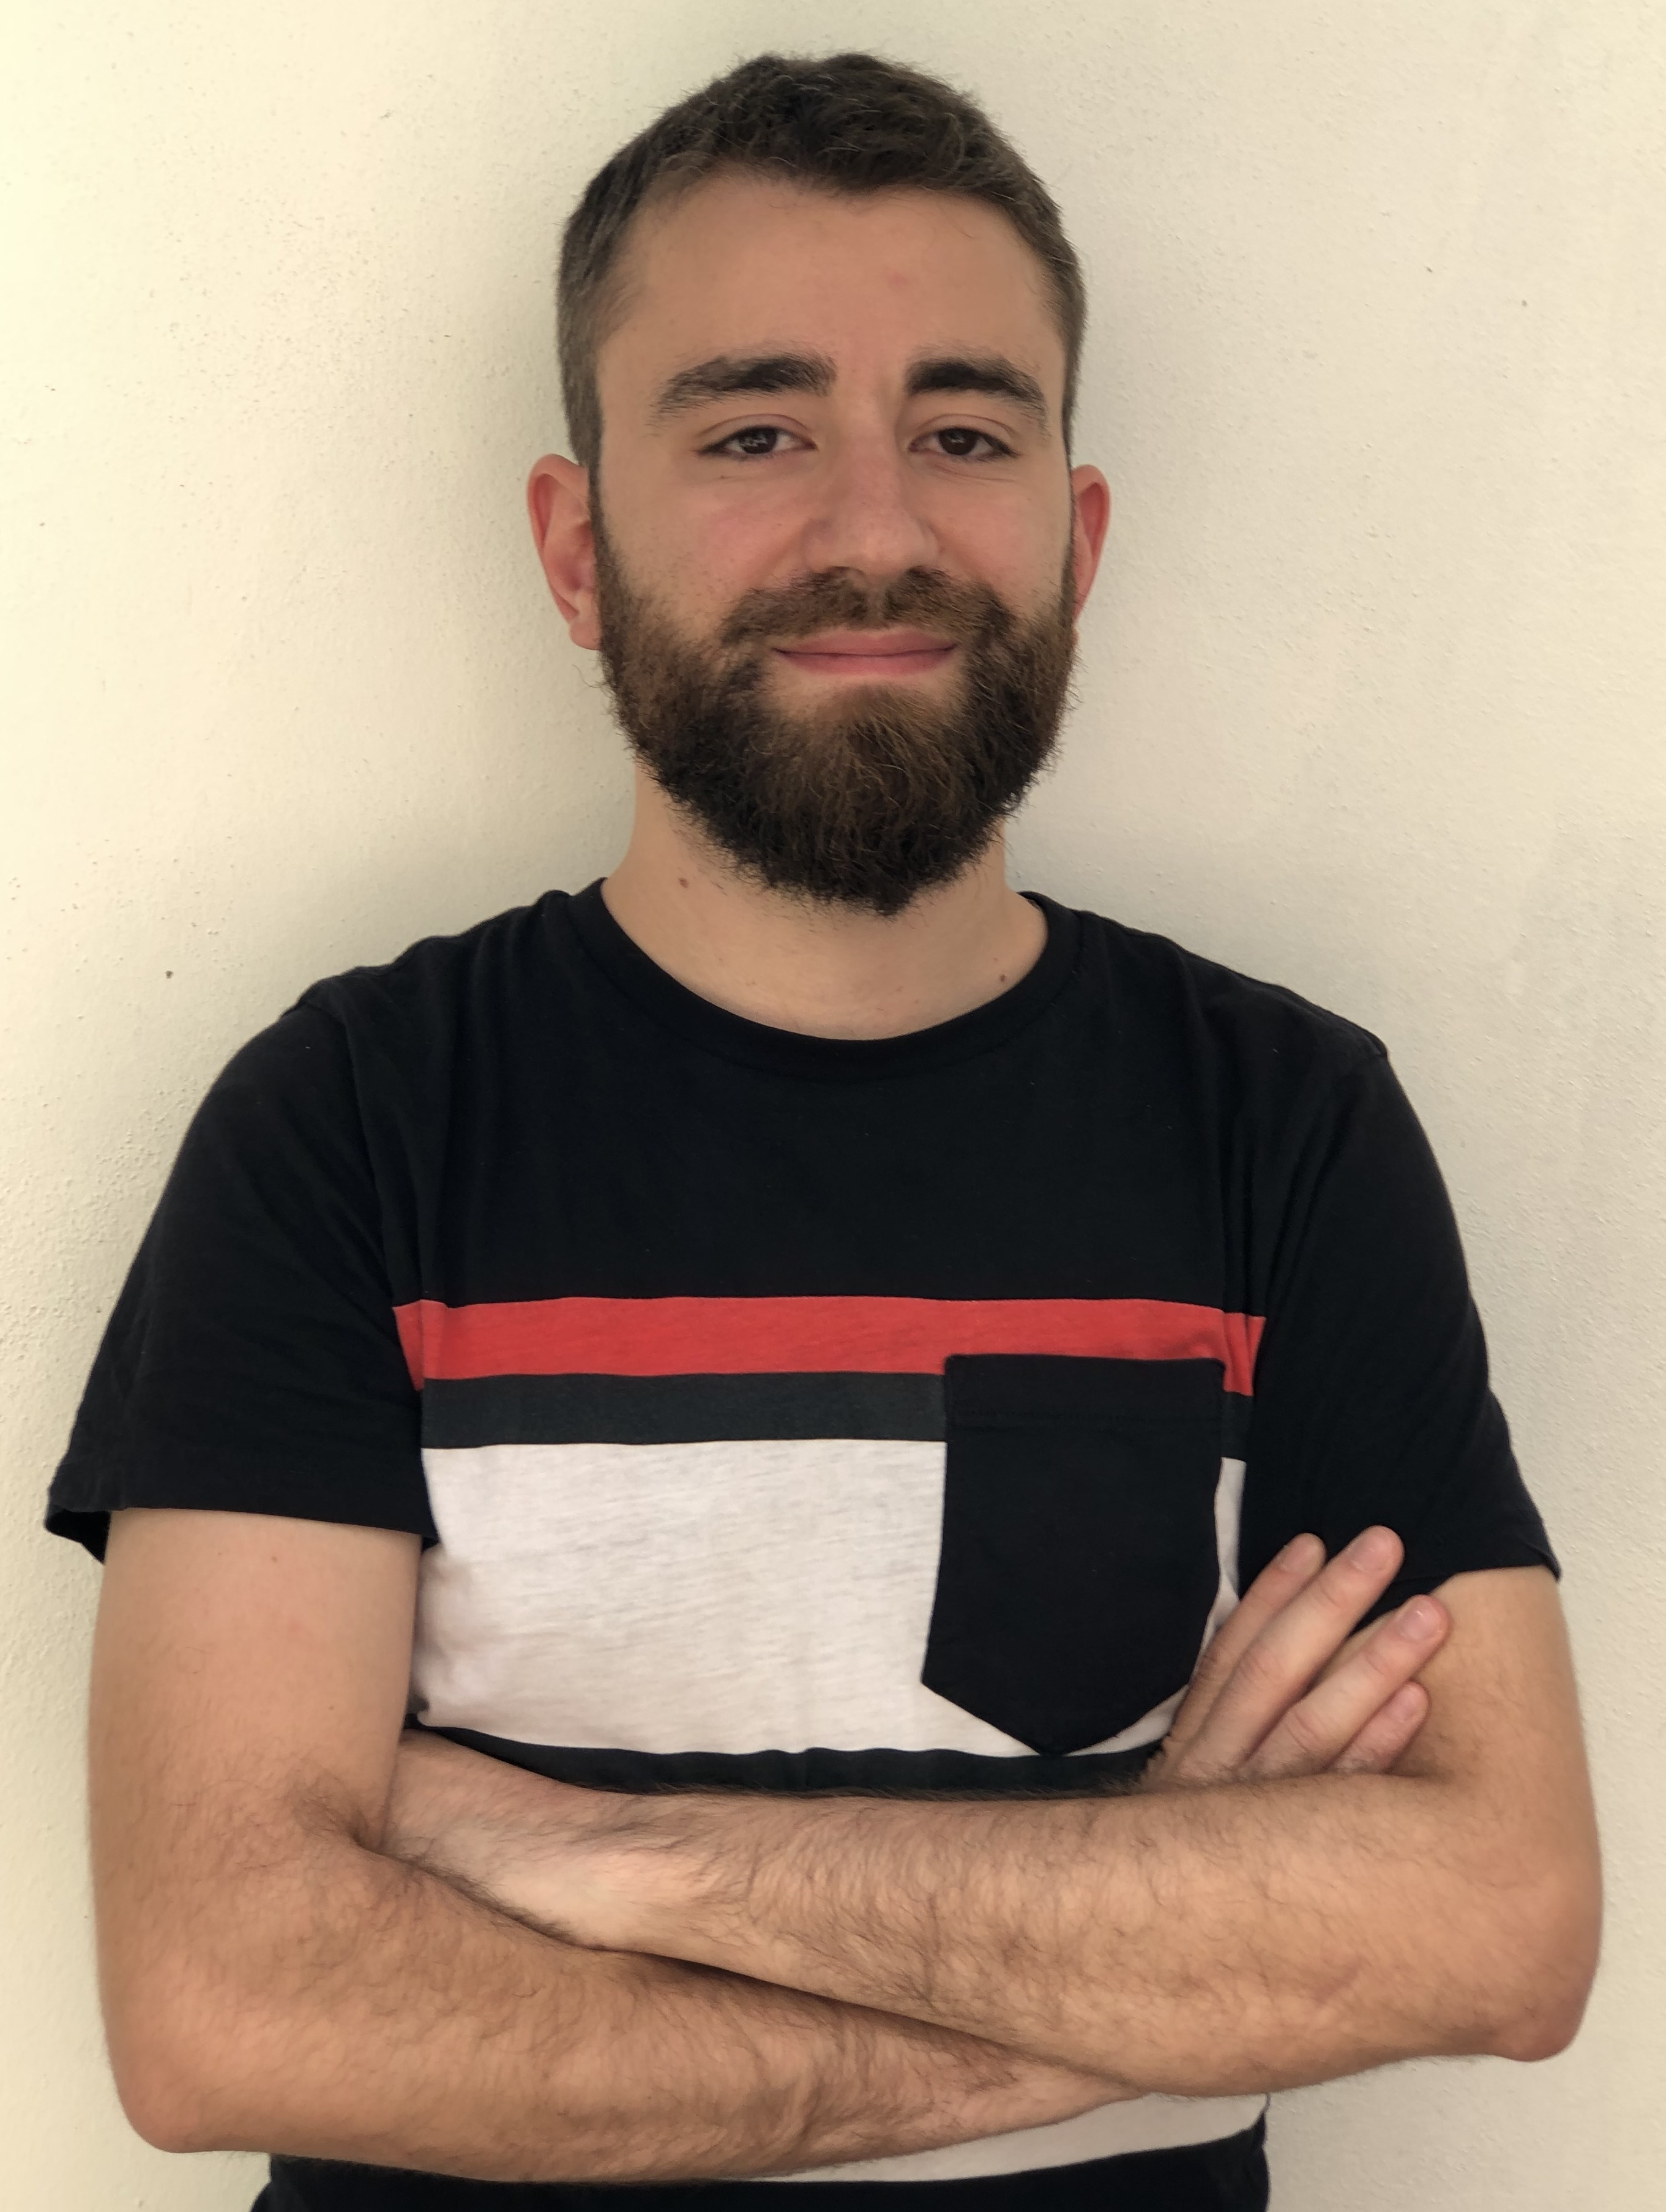
\includegraphics[width=0.9\columnwidth]{media/IMG_5751}\\[\baselineskip] % Your 
%photo
\small % Smaller font size
\textbf{Mail} \\
{\footnotesize\textit{ialoise@diag.uniroma1.it}} \\ 
\Sep

\textbf{Personal Site}\\
{\footnotesize\href{https://istinj.github.io}{https://istinj.github.io}}\\
\Sep

\textbf{LinkedIn} \\
{\footnotesize\href{https://goo.gl/NQvHbJ}{https://goo.gl/NQvHbJ}} \\ 
\Sep

\textbf{Birthday} \\
{\footnotesize May 21, 1991}
\vfill % Whitespace under this block to push it up under the photo
\end{flushright}
}

% ---------------------------------------------------------------------------- %
% ---------------------------------------------------------------------------- %
% ---------------------------------------------------------------------------- %

\begin{document}
\userinformation 
\framebreak 

% ---------------------------------------------------------------------------- %
%	HEADING
% ---------------------------------------------------------------------------- %
\cvheading{Irvin Aloise}
\cvsubheading{Ph.D. Candidate in \\Engineering in Computer Science}

% ---------------------------------------------------------------------------- %
%	EDUCATION
% ---------------------------------------------------------------------------- %
\CVSection{Education}

\CVItem{2017 - Oct 2020 (expected), Sapienza University of Rome}
  {\textbf{Ph.D. in Engineering in Computer Science} \\
    Research Topics: Mobile Robotics, Simultaneous Localization and Mapping, 
    Graph Optimization.\\
    Advisor: \textit{Prof. Dr. Giorgio Grisetti}.}

\CVItem{2019 - 2020, Rheinische Friedrich-Wilhelms-Universit\"at of Bonn}
{\textbf{Visiting Ph.D. Student} \\
  September 2019 - February 2020. \\
  Research Topics: 3D-Lidar SLAM, Sensor Calibration.\\
  Supervisor: \textit{Prof. Dr. Cyrill Stachniss}.}

\CVItem{2014 - 2017, Sapienza University of Rome}
  {\textbf{M.Sc. in Artificial Intelligence and Robotics} (in English) \\
  Thesis title: \textit{Extended Measurements in Pose-Graph Optimization}. \\
  Supervisor: \textit{Prof. Dr. Giorgio Grisetti} and \textit{Dominik 
  Schlegel}. \\
  Final grade: First Class with Honors ($\nicefrac{110}{110}$ cum laude).}

\CVItem{2010 - 2014, Sapienza University of Rome}
  {\textbf{B.Sc. in Electronic Engineering} (in Italian) \\
  Supervisor: \textit{Prof. Giuseppe Oriolo}}

\Sep % Extra whitespace after the end of a major section
\Sep % Extra whitespace after the end of a major section

% ---------------------------------------------------------------------------- %
%	PUBLICATIONS
% ---------------------------------------------------------------------------- %

\CVSection{Publications}

\CVItem{Chordal Based Error Function for 3D Pose-Graph Optimization}
       {\textbf{\small IEEE Robotics and Automation Letters (RA-L), 2019} 
  \\
  \underline{I. Aloise} and G. Grisetti \\ 
  DOI: \href{https://doi.org/10.1109/LRA.2019.2956456}{10.1109/LRA.2019.2956456} 
}

\CVItem{Systematic Handling of Heterogeneous Geometric Primitives in Graph-SLAM 
  Optimization}{\textbf{\small IEEE Robotics and Automation Letters (RA-L), 2019} 
  \\
  \underline{I. Aloise}, B. Della Corte, F. Nardi and G. Grisetti \\ 
  DOI: \href{https://doi.org/10.1109/LRA.2019.2918054}{10.1109/LRA.2019.2918054} 
}

\CVItem{Matrix Difference in Pose-Graph Optimization}{
  \textbf{ArXiv, 2018} \\
  \underline{I. Aloise} and G. Grisetti \\
  \href{https://arxiv.org/abs/1809.00952}{arXiv:1809.00952 [cs.RO]}}

\Sep % Extra whitespace after the end of a major section
\Sep % Extra whitespace after the end of a major section

% ---------------------------------------------------------------------------- %
% ---------------------------------------------------------------------------- %
% ---------------------------------------------------------------------------- %
\clearpage % Start a new page
\userinformation % Print your information in the left column
\framebreak % End of the first column

% ---------------------------------------------------------------------------- %
%	TEACHING
% ---------------------------------------------------------------------------- %

\CVSection{Teaching Activities}

\CVItem{September 2018 - June 2019, Sapienza University of Rome}
{\textbf{Teaching Assistant of Operating Systems - \textit{Sistemi Operativi}} 
  \\ Course held by Prof. G. Grisetti, B.Sc. in Engineering in Computer 
  Science, 
  6 ECTS credits.}

\Sep

\CVItem{November 2017 - June 2018, Sapienza University of Rome}
{\textbf{Teaching Assistant of Operating Systems - \textit{Sistemi Operativi}} 
  \\ Course held by Prof. G. Grisetti, B.Sc. in Engineering in Computer 
  Science, 6 ECTS credits.}

\Sep % Extra whitespace after the end of a major section
\Sep % Extra whitespace after the end of a major section

% ---------------------------------------------------------------------------- %
%	LANGUAGES
% ---------------------------------------------------------------------------- %
\CVSection{Languages}

\CVItem{Italian}{Mother-tongue}

\CVItem{English}{Advanced}

\Sep % Extra whitespace after the end of a major section
\Sep % Extra whitespace after the end of a major section

% ---------------------------------------------------------------------------- %
%	SKILLS
% ---------------------------------------------------------------------------- %
\CVSection{Skills}

\CVItem{Programming}
{C++, C, Octave, Matlab, Python, OpenGL and ImGui. }

%------------------------------------------------

\CVItem{Operating Systems}
{Ubuntu, Windows, MacOS}

%------------------------------------------------

\Sep % Extra whitespace after the end of a major section
\Sep % Extra whitespace after the end of a major section

% ---------------------------------------------------------------------------- %
%	INTERESTS
% ---------------------------------------------------------------------------- %

\CVSection{Interests}

\CVItem{Professional}{Mobile Robotics, SLAM, Sensor Calibration, Computer 
Vision, Autonomous Robotics, Machine Learning}

\CVItem{Personal}{Music, Cinema, Video-games, Technology, Photography, Motor 
Sports}

\Sep % Extra whitespace after the end of a major section
\Sep % Extra whitespace after the end of a major section

% ---------------------------------------------------------------------------- %
%	MISC PROJECTS
% ---------------------------------------------------------------------------- %

\CVSection{Personal Projects}
\CVItem{2019, Rheinische Friedrich-Wilhelms-Universit\"at of Bonn}{
  \textbf{Extrinsic Calibration between 3D-Lidar and Monocular Camera}}

\CVItem{2016, Sapienza Univesity of Rome, Exam project}{
  \textbf{Development of a Simulation Environment for Teleoperated Surgical 
  Tasks}}

\CVItem{2016, Sapienza University of Rome, Exam project}{
  \textbf{Analyzing Visualization Techniques for Convolutional Neural Neworks}}
\vspace{-10pt}

\CVItem{2015, Sapienza University of Rome, Exam project}{
  \textbf{A Third-Person Game Based on the \texttt{Three.js} Library}}

% ---------------------------------------------------------------------------- %
% ---------------------------------------------------------------------------- %
% ---------------------------------------------------------------------------- %
\clearpage % Start a new page
\userinformation % Print your information in the left column
\framebreak % End of the first column

\CVSection{References}

\vspace{15pt}
\begin{tabular}{>{\arraybackslash}p{0.45\linewidth}>{\arraybackslash}p{0.05\linewidth}>{\arraybackslash}p{0.45\linewidth}}
  %% \toprule
  %ia names
  \textbf{\color{RoyalBlue}Prof. Dr. Giorgio Grisetti} & {} &
  \textbf{\color{RoyalBlue}Prof. Dr. Cyrill Stachniss} \\
  % qualifications
  \textbf{Associate professor at Sapienza University of Rome} & {} &
  \textbf{Full professor at the University of Bonn} \\
  %ia lab/department
  Dept. of Computer, Control, and Management Engineering & {} &
  Head of the lab for Photogrammetry and Robotics \\
  %ia contacts - address
  {\footnotesize Via Ariosto 25, 00185, Rome, Italy} & {} &
  {\footnotesize Nussallee 15, 53115, Bonn, Germany} \\
  %ia contacts - mail
  {\footnotesize Mail: \href{mailto:grisetti@diag.uniroma1.it}{grisetti@diag.uniroma1.it}} & {} &
  {\footnotesize Mail: \href{mailto:cyrill.stachniss@igg.uni-bonn.de}{cyrill.stachniss@igg.uni-bonn.de}}
  %% \bottomrule
\end{tabular}


% ---------------------------------------------------------------------------- %
% ---------------------------------------------------------------------------- %
% ---------------------------------------------------------------------------- %
% ---------------------------------------------------------------------------- %

%% \vspace{20pt}
\vspace{3cm}
%\begin{flushleft}
%  {Rome, 2019.12.29}
%\end{flushleft}
\begin{flushright}
  {Irvin Aloise}
\end{flushright}


\end{document}
